\usepgflibrary{shapes.misc}
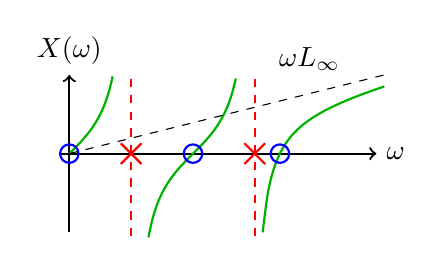
\begin{tikzpicture}[smooth, xscale=0.5, yscale=0.5]
% Achsen
\draw[->, thick] (-0.2,0) -- +(8,0) node[right] {$\omega$}; % Horizontal
\draw[->, thick] (0,-2) -- +(0,4) node[above] {$X(\omega)$}; % Vertikal

% Plots
\draw[color=green!70!black, thick] plot[domain=0:1.1] (\x,{tan(\x r)}); % Erster Tan
\draw[color=green!70!black, thick] plot[domain=2.01:4.23] (\x,{tan(\x r)}); % zweiter Tan
\draw[color=green!70!black, thick] plot[domain=4.91:8] (\x,{ (0.25 * \x) -1/(\x -4.6) }); % letzte kurve

% Poolstellen
\draw[dashed, thick, draw=red] (1.57,-2.1) -- +(0,4.2); % Poolstelle 1
\draw[dashed, thick, draw=red] (4.71,-2.1) -- +(0,4.2); % Poolstelle 2
\node[cross out, draw=red, thick] (wr1) at (1.57,0) {};
\node[cross out, draw=red, thick] at (4.71,0) {};


\draw[dashed] plot[domain=0:8] (\x, { 0.25 * \x});
\node (wL) at (6.1,2.4) {$\omega L_\infty$};

% Nullstellen
\node[rounded rectangle, draw=blue, thick] at(0,0) {};
\node[rounded rectangle, draw=blue, thick] at(3.141,0) {};
\node[rounded rectangle, draw=blue, thick] at(5.35,0) {};
\end{tikzpicture}